
\chapter{Unified Data Processing and Visualization}
\label{chap:tabgenie}

In \autoref{sec:tabgenie}, we make a step towards unified processing of \ac{d2t} generation datasets. We first convert the input data in 16 datasets of various formats and provenance (loosely related through the task of ``generating text based on data'') into a common tabular format. We take advantage of the unified access to the datasets for building \textsc{TabGenie}: a toolkit combining web interface, command-line interface and Python bindings for simplifying data visualization and processing. While data visualization helps us to get uncover contents of individual datasets, unified format opens up a posibility of streamlining datasets into \acp{plm} for multi-task training. Interactive mode, in which the model input can be modified on-the-fly, then helps us to to insights into the system behavior, the topic to which we will return in \autoref{chap:investigating}. In the end of the section, we present multiple real-world use-cases of our framework.


\section{TabGenie Toolkit}
\label{sec:tabgenie}

\begin{refbox}
    This section is based on the paper \emph{\textsc{TabGenie}: A Toolkit for Table-to-Text Generation} \cite{kasnerTabGenieToolkitTabletoText2023}, joint work with Ekaterina Garanina, Ondřej Plátek, and Ondřej Dušek. The work was published as a system demonstration in the Proceedings of the 61st Annual Meeting of the Association for Computational Linguistics (ACL 2023). The project was led by the author of the thesis, the other authors helped with implementing the framework and paper writing.
\end{refbox}


In this section, we present \textsc{TabGenie} -- a toolkit which enables researchers to explore, preprocess, and analyze a variety of \ac{d2t} generation datasets as tables with associated metadata. The web interface of \textsc{TabGenie} provides an interactive mode for debugging table-to-text generation models, facilitates side-by-side comparison of generated system outputs, and allows easy exports for manual analysis. \textsc{TabGenie} is also equipped with command line processing tools and Python bindings for unified dataset loading and processing. We release \textsc{TabGenie} as a Python package\footnote{\url{https://pypi.org/project/tabgenie/}} and provide its open-source code and a live demo through Github.\footnote{\url{https://github.com/kasnerz/tabgenie}}

\subsection{Motivation}
\label{sec:tabgenie:motivation}
In \autoref{tab:datasets}, we provided a representative, although not comprehensive, overview of research datasets for \ac{d2t} generation. As the number of datasets keeps growing and research keeps accelerating, researchers need to streamline their interactions with these datasets. However, each dataset comes with a different input format and task description, and the input data may not be easy to access and visualize.  Platforms such as HuggingFace Datasets \cite{lhoest2021datasets} or the GEM benchmark \cite{gehrmannGEMBenchmarkNatural2021}  provide a unified way to access the datasets, but they platforms still leave the majority of the data processing load on the user.

A key component missing from current \ac{d2t} tools is the possibility to visualize the input data and generated outputs. Visualization plays an important role in examining and evaluating scientific data \cite{Kehrer2013VisualizationAV} and can help researchers to make more informed design choices. A suitable interface can also encourage researchers to step away from unreliable automatic metrics \cite{gehrmannRepairingCrackedFoundation2022} and focus on manual error analysis \cite{van_miltenburg_underreporting_2021,van_miltenburg_barriers_2023}.

Along with that, demands for a \textit{unified input data format} have recently been raised with multi-task training for large language models (LLMs) \citep[\textit{inter alia}]{sanh2021multitask,scao2022bloom,ouyang2022TrainingLM}. Some works have used simple data linearization techniques for converting structured data to a textual format, in order to align it with the format used for other tasks \cite{xieUnifiedSKGUnifyingMultiTasking2022,tang2022mvp}. However, linearizations are using custom preprocessing code, leading to discrepancies between individual works.

To address these gaps, we present \textsc{TabGenie} -- a multi-purpose toolkit for interacting with \ac{d2t} generation datasets. The cornerstone of \textsc{TabGenie} is a \emph{unified data representation}. Each input represented is as a matrix of $m$ columns and $n$ rows consisting of individual cells accompanied with metadata. Building upon this representation, \textsc{TabGenie} then provides multiple features for unified workflows with table-to-text datasets, including:
\begin{enumerate}
    \item visualizing individual dataset examples in the tabular format,
    \item interacting with table-to-text generation systems in real-time,
    \item comparing generated system outputs,
    \item loading and preprocessing data for downstream tasks,
    \item exporting examples and generating spreadsheets for manual error analysis,
\end{enumerate}

\subsection{Data}
\label{sec:tabgenie:data}

\begin{figure*}[t]
    \centering
    \setlength{\fboxsep}{0pt}\fcolorbox{gray!20}{white}{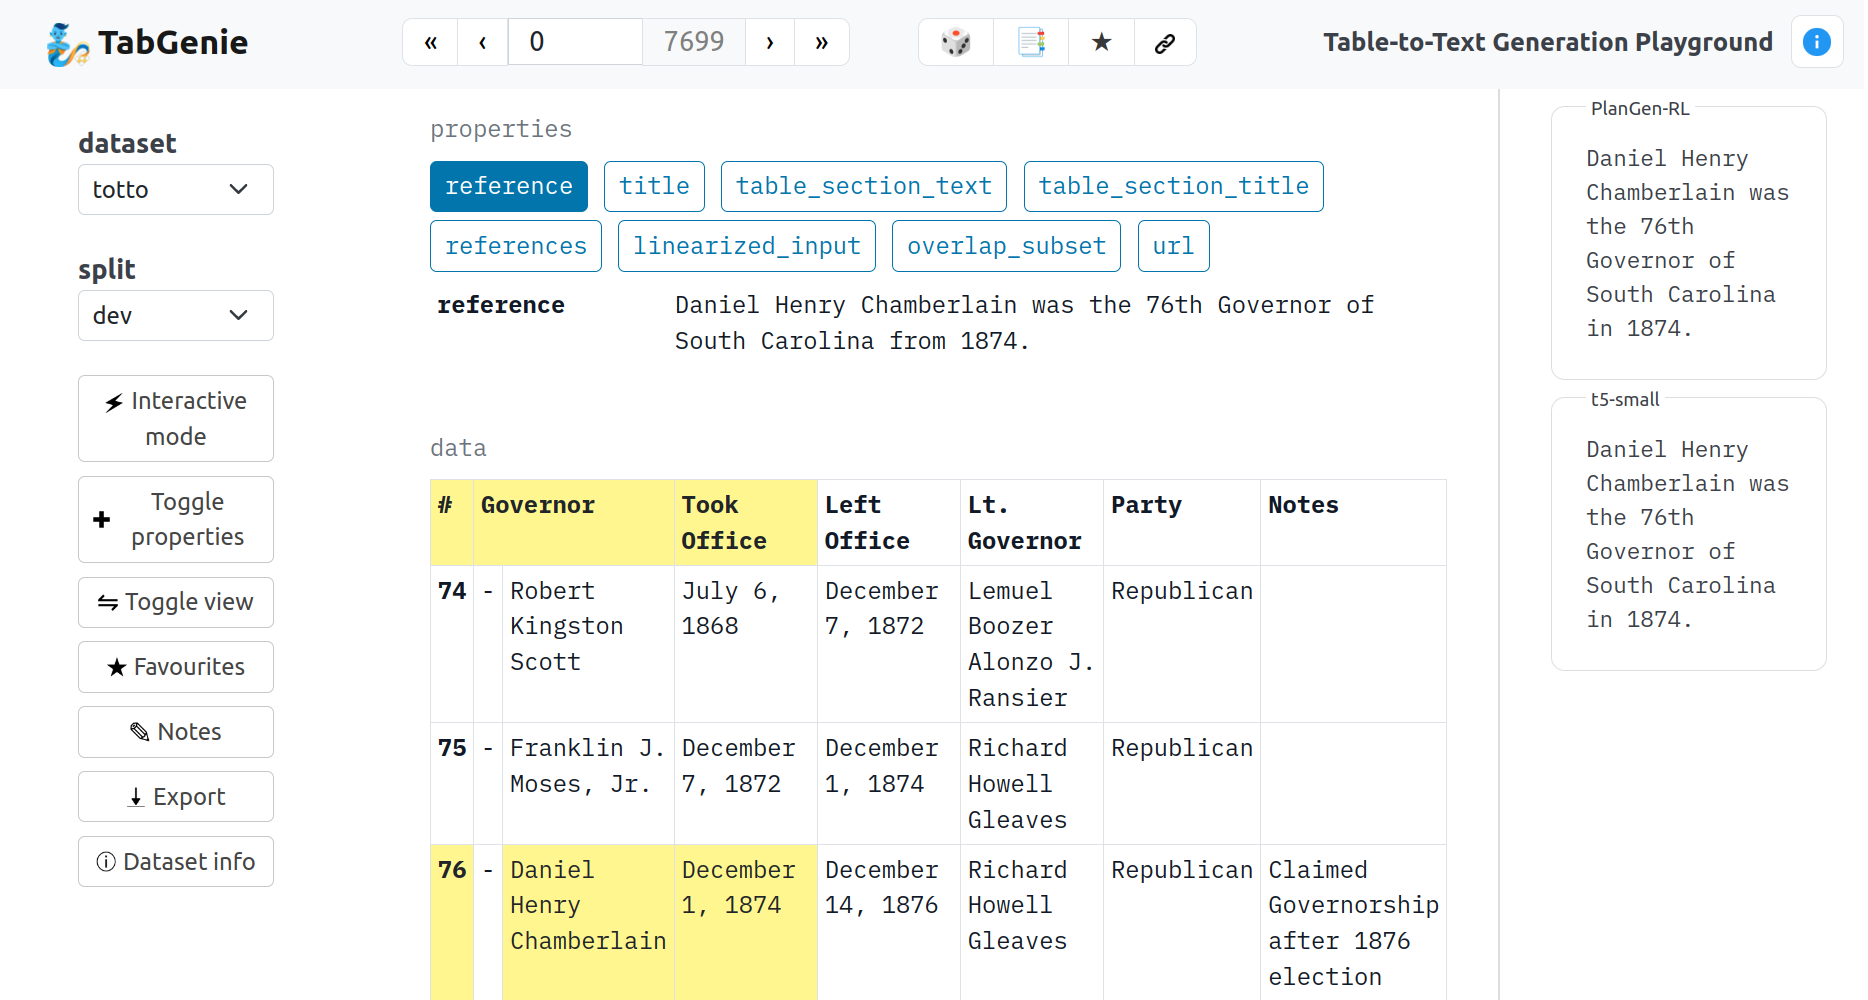
\includegraphics[width=1.0\textwidth]{img/tabgenie_web.png}}
    \caption{The web interface of \textsc{TabGenie}. The \emph{left panel} and the \emph{navigation bar} contains user controls; the \emph{center panel} shows table properties and table content; the \emph{right panel} contains system outputs.}
    \label{fig:tabgenie:web}
\end{figure*}


\paragraph{Unifying Data Format}
Our \ac{d2t} generation datasets contain three high-level input data formats: tables, \acs{rdf}\glsunset{rdf} triples, and key-value pairs. We note that converting the latter two to tabular format requires only minimal changes to the data structure while allowing a unified data representation and visualization. The unified representation narrows down the task to generating description for a tabular data, i.e., \emph{table-to-text generation} \cite{parikhToTToControlledTableToText2020,liuPLOGTabletoLogicPretraining2022,gongTableGPTFewshotTabletoText2020}.

\paragraph{Tabular Inputs} We define a \textit{table} as a two-dimensional matrix with $m$ columns and $n$ rows, which together define a grid of $m \times n$ cells. Each cell contains a (possibly empty) text string. A continuous sequence of cells $\{c_{i}, \ldots, c_{i+k}\}$ from the same row or column may be merged, in which case the values of $\{c_{i+1},\ldots,c_{i+k}\}$ are linked to the value of $c_{i}$.  A cell may be optionally marked as a \textit{heading}, which is represented as an additional property of the cell.\footnote{The headings are typically located in the first row or column, but may also span multiple rows or columns and may not be adjacent.} To better accommodate the format of datasets such as ToTTo \cite{parikhToTToControlledTableToText2020} or HiTab \cite{chengHiTabHierarchicalTable2021}, we also allow individual cells to be \textit{highlighted}. Highlighted cells are assumed to be preselected for generating the output description. The tables may be accompanied with an additional set of properties (see \autoref{fig:tabgenie:web})\footnote{An example of such a property is a \textit{``title''} of the table in WikiBio \cite{lebretNeuralTextGeneration2016} or a \textit{``category''} in WebNLG \cite{gardentWebNLGChallengeGenerating2017}.}, which we represent as key-value pairs alongside the table. The properties may be used for generating the table description.

\paragraph{Data Transformation} Although we mostly preserve the original structure of the data, we make a few minor changes to datasets which do not immediately adhere to the tabular format:

\begin{itemize}
    \item For graph-to-text datasets, we format each triple as a row, using three columns labeled \textit{subject}, \textit{predicate}, and \textit{object}.
    \item For key-value datasets, we use two-column format, with keys used as row headings in the first column.
    \item For SportSett:Basketball \cite{thomson2020sportsett}, we merge the \textit{box score} and \textit{line score} tables and add appropriate headings where necessary.
\end{itemize}

% Moreover, for ToTTo \citep{parikhToTToControlledTableToText2020}, we also provide our custom, improved header cells highlighting (details are given in Appendix \ref{appendix:totto_highlights}).


\paragraph{Datasets}
We include 16 datasets listed in \autoref{tab:datasets} in \textsc{TabGenie}, covering many subtasks of \ac{d2t} generation. All the datasets are available under a permissive open-source license. To ease the data distribution, we load all the datasets using the Huggingface \texttt{datasets} package \cite{lhoest2021datasets}, which comes equipped with a data downloader. We publicly added to Huggingface \texttt{datasets} 9 out of 16 datasets which were not yet available.\footnote{See \url{https://huggingface.co/datasets?search=kasnerz}} A custom dataset can be added to \textsc{TabGenie} by simple sub-classing the data loader class and overriding the method for processing individual entries.

\subsection{Web Interface}
\label{sec:tabgenie:web}

\textsc{TabGenie} offers a way to interact with the datasets through the \textit{web interface}. The interface features a single-page layout with three panels containing user controls, input data, and system outputs (see \autoref{fig:tabgenie:web}).

\paragraph{Content Exploration} \textsc{TabGenie} renders input data as HTML tables, providing superior visualizations to existing data viewers, especially in the case of large and hierarchical tables.\footnote{Compare, e.g., with the ToTTo dataset in Huggingface Datasets for which the table is provided in a single field called \textit{``table''}: \url{https://huggingface.co/datasets/totto}.} Users can navigate through individual examples in the dataset sequentially, access an example using its index, or go to a random example. The users can add notes to examples and mark examples as favorites for accessing them later. The interface also shows the information about the dataset (such as its description, version, homepage, and license) and provides an option to export the individual examples.

\paragraph{Interactive Mode} In the interactive mode, the user can modify the input data and observe how changes influence model outputs. We assume that the model is running externally and provides access through an \acs{api} which is queried by \textsc{TabGenie}. The user can highlight different cells, edit cell contents, and edit parameters of the downstream processor.

% For example,  The contents of a table are processed by a processing \textit{pipeline}. This pipeline takes table contents and properties as input, processes them with a sequence of modules, and outputs HTML code. The modules are custom Python programs which may be re-used across the pipelines.

% \textsc{TabGenie} currently provides two basic pipelines: (1) calling a generative language model through an API with a custom prompt, and (2) generating graph visualizations of RDF triples. We describe a case-study for the model API pipeline in §\ref{sec:cs:prompting}. Users can easily add custom pipelines by following the instructions in the project repository.

\paragraph{Pre-generated Outputs} \textsc{TabGenie} also allows to visualize static pre-generated outputs. These are loaded in the JSONL\footnote{\url{https://jsonlines.org}} format from a specified directory and displayed similarly to model-generated outputs from the interactive mode. Multiple outputs can be displayed alongside a specific example, allowing to compare outputs from multiple systems.


\subsection{Developer Tools}
\label{sec:tabgenie:developer}
Beside the web interface, \textsc{TabGenie} also provides more developer-friendly access through Python bindings and a command-line interface. Both of these interfaces aim to simplify dataset preprocessing in downstream tasks. The key benefit of using \textsc{TabGenie} is that it provides streamlined access to data in a consistent format, removing the need for dataset-specific code for extracting information such as table properties, references, or individual cell values.



\paragraph{Python Bindings} \textsc{TabGenie} can replace custom preprocessing code in Python codebases. With a single unified interface for all the datasets, the \textsc{TabGenie} wrapper class allows to:
\begin{itemize}
    \item load a dataset from the Huggingface Datasets or from a local folder,
    \item access individual table cells and their properties,
    \item linearize tables using pre-defined or custom functions,
    \item prepare the Huggingface \texttt{Dataset} objects for downstream processing.
\end{itemize}
\textsc{TabGenie} can be installed as a Python package, making the integration simple and intuitive.

\paragraph{Command-line Tools} \textsc{TabGenie} supports several basic commands via command line:
\begin{itemize}
    \item \textbf{Run} The \texttt{tabgenie run} command launches the local web server, mimicking the behavior of \texttt{flask run}.

          \noindent Example usage:
          % \begin{noindent}
\begin{bash}
tabgenie run --port=8890 --host="0.0.0.0"
\end{bash}
% \end{noindent}
    \item \textbf{Export} The \texttt{tabgenie export} command enables batch exporting of the dataset. The supported formats are \texttt{xlsx}, \texttt{html}, \texttt{json}, \texttt{txt}, and \texttt{csv}. Except for \texttt{csv}, table properties can be exported along with the table content.

          \noindent Example usage:
          % \begin{noindent}
\begin{bash}
tabgenie export --dataset "webnlg" \
    --split "dev" \
    --out_dir "export/datasets/webnlg" \
    --export_format "xlsx"
\end{bash}
% \end{noindent}
          \noindent Export can also be done in the web interface.
    \item \textbf{Spreadsheet} For error analysis, it is common to select $N$ random examples from the dataset along with the system outputs and manually annotate them with error categories. The \texttt{tabgenie sheet} command generates a suitable spreadsheet for this procedure.

          \noindent Example usage:
          % \begin{noindent}
\begin{bash}
tabgenie sheet --dataset "webnlg" \
    --split "dev" \
    --in_file "out-t5-base.jsonl" \
    --out_file "analysis_webnlg.xlsx" \
    --count 50
    \end{bash}
% \end{noindent}
\end{itemize}